\chapter{Lecture 30 - More Boundary Value Problem Examples}
\label{ch:lec30n}
\section{Objectives}
The objectives of this lecture are to:
\begin{itemize}
\item Illustrate the use of Robin boundary conditions with another example.
\item Show how to solve BVPs with an unknown parameter with \lstinline[style=myMatlab]{bvp5c}.
\end{itemize}
\setcounter{lstannotation}{0}

\section{Example Problem \#1}
\begin{marginfigure}
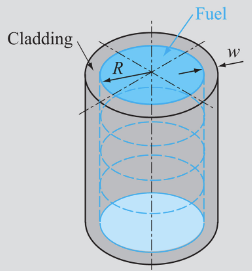
\includegraphics{lec30n-ex1-schematic.png}
\caption{A typical nuclear reactor fuel pin.}
\label{fig:lec30n-ex1-schematic}
\end{marginfigure}
Fuel rods of a nuclear reactor are cylindrical structures with the fuel retained inside cladding material, as shown in the figure.  The fuel causes heat to be generated by nuclear reactions withing the cylinder as well as in the cladding.\sidenote{The former is energy produced by fission, the latter is energy deposited by fission-induced photons within the cladding material.} The outer surface of the cladding is cooled by flowing water at $T_{\infty}=473$K with heat transfer coefficient of $h=10^4\ \text{W/m}^2\text{-K}$.  The thermal conductivity of the cladding material is $k=16.75 \ \text{W/m-K}$.  The dimensions of the fuel rod are $R=1.5\times 10^{-2}\text{ m}$, and $w=3.0\times 10^{-3}\text{ m}$. The temperature distribution in the cladding is determined by the solution of the following boundary value problem.  
\begin{table}
\begin{tabular}{l l}
ODE: & $\frac{1}{r}\frac{d}{dr}\left(rk\frac{dT}{dr}\right)=-10^8\frac{e^{-r/R}}{r}, \ \  R < r < R+w $ \\
BCs: & $\frac{dT}{dr}\Bigl|_{r=R}=-\frac{6.32\times 10^5}{k}, \ \ \frac{dT}{dr}\Bigl|_{r=R+w}=-\frac{h}{k}\left(T(r+w)-T_{\infty}\right)$ \\
\end{tabular}
\end{table}
We will use MATLAB's built-in function \lstinline[style=myMatlab]{bvp5c} to solve the boundary value problem and plot the temperature distribution in the cladding as a function of radial position, $r$.

First, we must transform the governing equation:
\begin{align*}
\frac{1}{r}\frac{d}{dr}\left(rk\frac{dT}{dr}\right) &=-10^8\frac{e^{-r/R}}{r} \\
\frac{d}{dr}\left(rk\frac{dT}{dr}\right)&=-10^8e^{-r/R} \\
k\frac{dT}{dr}+rk\frac{d^2T}{dr^2} &= -10^8e^{-r/R} \\
\frac{d^2T}{dr^2}+\frac{1}{r}\frac{dT}{dr} &= -\frac{10^8e^{-r/R}}{rk}
\end{align*}
\marginnote[-4.0cm]{

\vspace{0.1cm}

\noindent The original governing equation.

\vspace{0.5cm}

\noindent Multiply both sides by $r$.

\vspace{0.5cm}

\noindent Apply the product rule to the left-hand side.

\vspace{0.5cm}

\noindent Divide both sides by $rk$ and re-arrange terms.

}

